\documentclass[11pt, a4paper]{article}

% PAQUETES BÁSICOS
\usepackage[utf8]{inputenc} % Codificación de entrada UTF-8
\usepackage[T1]{fontenc}    % Codificación de fuentes
\usepackage[spanish,es-tabla]{babel} % Idioma español y tablas
\usepackage{csquotes}       % Para comillas contextuales
\usepackage{geometry}       % Para márgenes
\geometry{a4paper, margin=2.5cm} % Configuración de márgenes
\usepackage{graphicx}       % Para incluir imágenes
\usepackage{amsmath}        % Para fórmulas matemáticas avanzadas
\usepackage{amssymb}        % Símbolos matemáticos
\usepackage{float}          % Para controlar la posición de flotantes [H]
\usepackage{caption}        % Mejor control de captions
\usepackage{setspace}       % Para interlineado
\onehalfspacing
\usepackage{url}            % Para comando \url
\usepackage[hidelinks]{hyperref} % Para enlaces clicables (sin los recuadros de color)

\hypersetup{
    colorlinks=true,
    linkcolor=blue,
    filecolor=magenta,      
    urlcolor=cyan,
    pdftitle={The Orchestrator-Agent Framework (OAF)},
    pdfpagemode=FullScreen,
    breaklinks=true
}

% --- Información del Documento ---
\title{The Orchestrator-Agent Framework (OAF): A Systematic Methodology for Human-AI Collaborative Research in Data Science}
\author{Arian Pedroza Celis \\ \textit{Universidad Nacional Rosario Castellanos}}
\date{\today}

\begin{document}

\maketitle

\begin{abstract}
\noindent
El advenimiento de los sistemas de IA agéntica promete una aceleración sin precedentes en la investigación. Sin embargo, su aplicación, a menudo ad-hoc y no estructurada, introduce riesgos significativos como la ineficiencia, la falta de reproducibilidad y el sesgo de automatización, donde el juicio humano cede ante resultados de IA plausibles pero no verificados. Este paper introduce el \textbf{Orchestrator-Agent Framework (OAF)}, una metodología sistemática diseñada para transformar la colaboración humano-IA en una simbiosis cognitiva robusta. Inspirado en la teoría del proceso dual, el OAF postula una arquitectura funcionalmente distinta: (1) un \textbf{Agente de Deep Research (DR)}, análogo al ''Sistema 1'' rápido e intuitivo, que actúa como un motor de exploración y generación de hipótesis autónomo; y (2) un \textbf{Orquestador humano}, el ''Sistema 2'' lento y deliberativo, cuyo rol formal es validar críticamente, gobernar estratégicamente y mitigar los errores del Agente. La interacción es gobernada por un \textbf{Ciclo de Iteración Universal (UIC)} que, al externalizar y hacer auditable el proceso de investigación, aborda directamente las causas de la crisis de reproducibilidad. A través de un caso de estudio post-mortem y la validación de resultados de investigaciones análogas que demuestran la compresión de más de una década de trabajo en días (Cao et al., 2025), argumentamos que el OAF no solo previene anti-patrones comunes, sino que optimiza la carga cognitiva del investigador, permitiendo una ciencia de datos más rápida, profunda y confiable.
\end{abstract}

\tableofcontents
\newpage

% --- INICIO DEL CUERPO DEL PAPER ---

\section{Introducción: De la Promesa Generativa al Caos Agéntico}
\label{sec:introduccion}

El campo de la inteligencia artificial se encuentra en una encrucijada crítica, una que redefinirá no solo la computación, sino el futuro mismo de la investigación y la resolución de problemas complejos. Hemos transitado de la asombrosa capacidad de los modelos generativos a la emergencia explosiva de la IA agéntica. Esta nueva clase de sistemas incluye no solo chatbots conversacionales avanzados, sino también \textbf{motores de investigación profunda (Deep Research)}, capaces de escanear y sintetizar información de cientos de fuentes web y papers académicos. Esta transición, descrita como el paso de ''sistemas generativos a sistemas de acción'' \cite{xi2023}, promete una aceleración sin precedentes, pero para el científico de datos y el investigador, también ha traído consigo un nuevo tipo de caos.

Para el profesional que se sumerge en proyectos complejos, la proliferación de agentes de IA puede ser una bendición y una maldición. La tentación es usarlos de forma ad-hoc, lanzando prompts aislados y esperando una revelación. Sin embargo, este enfoque anárquico no solo es ineficiente, sino que nos arrastra hacia \textbf{anti-patrones insidiosos}: desde la ''cacería heroica de datos'' que devora meses de tiempo, hasta la ''parálisis por análisis'' que ahoga el insight en un mar de visualizaciones. En el peor de los casos, la falta de una supervisión rigurosa conduce a ''alucinaciones'' y sesgos que socavan la confianza y la integridad de la investigación.

Este paper se propone como un manifiesto y una hoja de ruta. Introducimos el \textbf{Orchestrator-Agent Framework (OAF)}, una metodología sistemática, rigurosa y transparente, diseñada para gobernar y potenciar la inteligencia agéntica. Nuestra tesis central es que la colaboración más efectiva y segura entre humanos e IA se logra a través de una arquitectura de roles especializados y un bucle de retroalimentación dinámico. Ofrecemos un marco que:
\begin{enumerate}
    \item \textbf{Optimiza Recursos Cognitivos:} Protege al investigador humano de la sobrecarga.
    \item \textbf{Acelera la Velocidad de Investigación:} Reduce drásticamente los tiempos de las fases críticas.
    \item \textbf{Maximiza la Eficiencia Computacional:} Fomenta el uso estratégico de los recursos de IA, priorizando el ROI.
    \item \textbf{Incrementa la Robustez y Seguridad:} Mitiga sistemáticamente las limitaciones intrínsecas de los agentes de IA.
\end{enumerate}
Al exponer la estructura subyacente y los ejemplos de nuestros propios prompts, este documento ofrece no solo un marco teórico robusto, sino una metodología práctica y replicable para una nueva era de investigación en ciencia de datos.

\section{Fundamentos Conceptuales: Arquitecturas Cognitivas y Tecnológicas}
\label{sec:fundamentos}

El Orchestrator-Agent Framework (OAF) no es una construcción de ingeniería arbitraria, sino una arquitectura deliberada que emerge en la intersección de la ciencia cognitiva y la inteligencia artificial. 

\subsection{El Modelo Cognitivo de Proceso Dual: El ''Porqué'' del OAF}
La teoría del proceso dual de Daniel Kahneman \cite{kahneman2011} es fundamental para entender la lógica del OAF. El \textbf{Sistema 1} de Kahneman es rápido e intuitivo pero propenso a sesgos, mientras que el \textbf{Sistema 2} es lento y lógico pero propenso a la ''pereza'' cognitiva. El OAF no solo replica este modelo, sino que lo evoluciona, creando una arquitectura de inteligencia híbrida.

\begin{itemize}
    \item \textbf{El Agente de Deep Research (DR) como Sistema 1:}
    Este componente no es un chatbot conversacional, sino una herramienta de investigación profunda y autónoma. Actúa como un ''Sistema 1'' sobrealimentado: extraordinariamente rápido en la generación de hipótesis y la recopilación de información, pero inherentemente poco fiable sin supervisión, siendo vulnerable a ''ilusiones cognitivas'' como la alucinación factual y la amplificación de sesgos \cite{aws2024}.
    
    \item \textbf{El Sistema Orquestador como un Híbrido de Sistema 2:}
    Aquí reside la innovación central del OAF. El rol del ''Sistema 2'' no es ejercido únicamente por el humano, sino por un \textbf{sistema híbrido y simbiótico} compuesto por:
    \begin{enumerate}
        \item \textbf{El Componente IA del Orquestador (El ''Motor Deliberativo''):} Un LLM con una vasta ventana de contexto (ej. Gemini 2.5 Pro) que aporta la potencia computacional para el pensamiento lento y esforzado a gran escala. Su función es ingerir y analizar los complejos informes del Agente DR, mantener el contexto completo del proyecto y proponer borradores de diagnósticos y estrategias.
        \item \textbf{El Componente Humano (El ''Director Estratégico''):} Actúa como el árbitro final del juicio, la ética y la estrategia. Su función no es realizar el análisis masivo, sino \textbf{gobernar} al motor deliberativo: valida sus conclusiones, corrige su razonamiento, inyecta el contexto de negocio y toma la decisión estratégica final.
    \end{enumerate}
\end{itemize}

Esta arquitectura híbrida convierte un diálogo mental interno en un proceso explícito y auditable. Actúa como una defensa estructural contra el ''sesgo de automatización'', ya que el humano no está validando a un agente solitario, sino que está colaborando con su propio ''co-piloto'' de IA para supervisar al agente de campo (el DR). Se fuerza una deliberación de múltiples capas, algo crucial en dominios de alto riesgo como la investigación científica o el análisis financiero.
\subsection{Los Motores Tecnológicos Subyacentes: El ''Cómo'' del OAF}
La capacidad del OAF para operar de esta manera se basa en dos avances tecnológicos que han tenido un desarrollo tecnológico secuencial y, finalmente complementario que potencian a sus componentes.\begin{itemize}
    \item \textbf{A. El ''Cerebro'' - Transformers y Auto-Atención \cite{vaswani2017}:} La existencia de los LLMs modernos se debe a la arquitectura Transformer. Su innovación clave fue el mecanismo de auto-atención, que permite al modelo sopesar la importancia de todas las palabras en una secuencia simultáneamente, rompiendo las limitaciones de las arquitecturas anteriores y permitiendo una escala masiva. Esta tecnología es el ''cerebro'' que potencia a ambos componentes del OAF:
    \begin{enumerate}
        \item \textbf{Para el Orquestador:} (implementado como un chatbot de gran contexto), la arquitectura Transformer le otorga la capacidad de razonar sobre los vastos y complejos informes proporcionados por el Agente.
        \item \textbf{Para el Agente DR:} le da la habilidad de comprender y sintetizar el lenguaje de los cientos de documentos que analiza durante sus misiones de investigación.
    \end{enumerate}
    \item \textbf{B. Los ''Brazos y Piernas'' - ReAct \cite{yao2022}:} Si el Transformer proporcionó la capacidad de ''pensar'', el paradigma ReAct (Reason + Act) le dio al Agente DR la capacidad de ''hacer''. ReAct sinergiza el razonamiento con la acción, permitiendo al LLM generar trazas de pensamiento y acciones (como usar una API de búsqueda) de manera intercalada. Esta capacidad de actuar para interactuar con herramientas externas es lo que dota al Agente DR de sus ''brazos y piernas'' para explorar el entorno digital. Ancla su proceso de investigación en la realidad, permitiéndole verificar hechos, obtener información actualizada y transformar la investigación de un ejercicio pasivo a una exploración activa y autónoma.
\end{itemize}

\section{Metodología: Componentes y Dinámicas del Framework OAF}
\label{sec:metodologia}

El Orchestrator-Agent Framework (OAF) no es una colección de ''buenas prácticas'', sino una metodología sistemática diseñada como un antídoto directo a los anti-patrones que plagan la investigación no estructurada con IA. Cada componente y cada dinámica del OAF existe para justificar su propósito: transformar el flujo de trabajo de un arte incierto a una ciencia eficiente y replicable. Esta sección desglosa la arquitectura del OAF, argumentando cómo cada elemento contribuye a la optimización de recursos y a la profundización del insight.

\subsection{Arquitectura de Componentes: La División Deliberada del Trabajo Cognitivo}
El OAF postula una división de trabajo deliberada para mitigar la sobrecarga cognitiva del investigador solitario. El \textbf{Orquestador} gobierna y el \textbf{Agente DR} explora. Sin el rol formal del Orquestador, el investigador es vulnerable al sesgo de automatización. Sin un Agente formalmente comisionado, la investigación se estanca en la ''cacería heroica de datos''.

\subsection{Dinámica Central: El Ciclo de Iteración Universal (UIC)}
El UIC es el motor que impulsa el proyecto. Sin un ciclo explícito, la investigación se vuelve una serie de acciones inconexas. El UIC impone una estructura donde cada acción es evaluada y cada evaluación informa la siguiente, creando un rastro de decisiones auditable. La interacción entre los componentes no es una simple conversación, sino un proceso riguroso y cíclico. El UIC es el motor que impulsa el proyecto, asegurando que cada paso sea deliberado y productivo.
\begin{figure}[H]
    \centering
    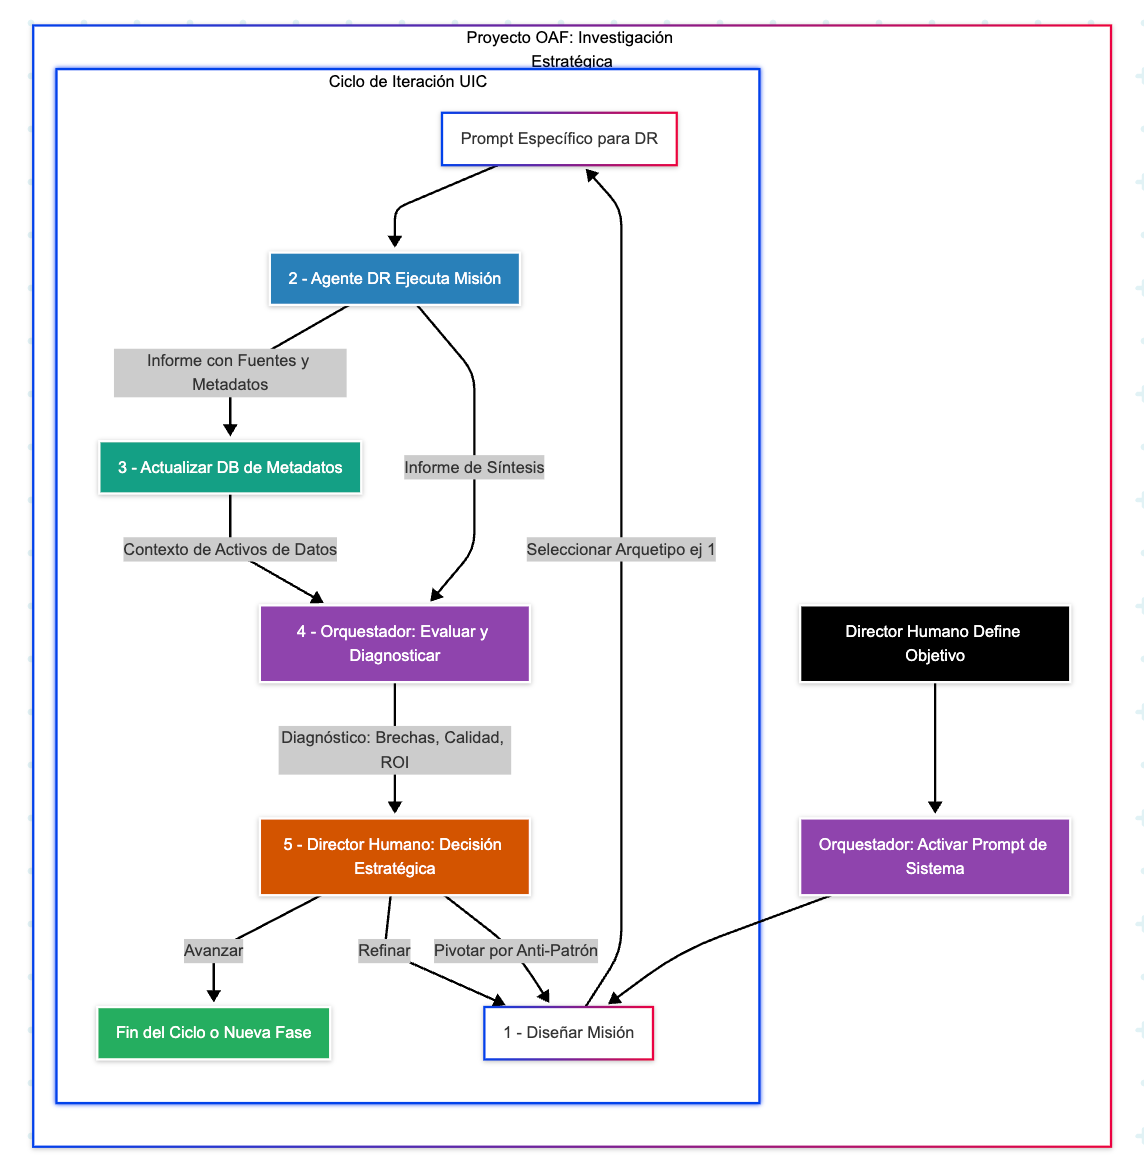
\includegraphics[width=\textwidth]{oaf_diagram.png}
    \caption{Diagrama de Flujo del Ciclo de Iteración Universal (UIC) del OAF.}
    \label{fig:oaf_diagram}
\end{figure}

\subsection{La Memoria del Sistema: La Base de Datos de Metadatos}
Quizás el ejemplo más potente de la eficiencia del OAF radica en su gestión de la información externa. El OAF utiliza una Base de Datos de Metadatos, poblada por el Agente DR, como una memoria externa y consultable. Esto convierte la recolección de datos de una búsqueda a ciegas en una serie de movimientos estratégicos, donde el Orquestador puede identificar brechas y proponer búsquedas de precisión (zoom in) o comparativas (zoom out).

\subsection{El enfoque Caótico (Sin OAF): } El investigador encuentra decenas de fuentes. Guarda enlaces en un navegador, descarga archivos en una carpeta desordenada. La ''memoria'' del proyecto es frágil y reside enteramente en la mente del investigador. Al querer combinar datos, debe recordar manualmente qué archivo contenía qué variables, de qué periodo de tiempo, y con qué nivel de calidad. Este proceso es propenso a errores y consume una cantidad desproporcionada de carga cognitiva en tareas de bajo nivel. 

\subsection{La Memoria del Sistema: La Base de Datos de Metadatos como Acelerador Estratégico}
\label{sec:metodologia_memoria}

Quizás el ejemplo más potente de la eficiencia del OAF radica en su gestión de la información externa, específicamente a través de la creación y uso de una base de datos de metadatos.

\textbf{El Enfoque Caótico (Sin OAF):} El investigador encuentra decenas de fuentes. Guarda enlaces en un navegador y descarga archivos en una carpeta desordenada. La ''memoria'' del proyecto es frágil, desestructurada y reside enteramente en la mente del investigador. Al querer combinar datos, debe recordar manualmente qué archivo contenía qué variables y de qué periodo. Este proceso es propenso a errores y consume una cantidad desproporcionada de carga cognitiva en tareas de bajo nivel.

\textbf{El Enfoque Estructurado (Con OAF):} El OAF transforma este proceso en un ciclo de inteligencia de datos sistemático y auditable:

\begin{enumerate}
    \item \textbf{Creación (Arquetipo \#1):} El Orquestador comisiona una misión DR con el ''Cosechador de Datos''. El Agente devuelve una tabla Markdown con una lista curada de datasets relevantes y sus metadatos clave (nombre, URL, formato, descripción, variables, cobertura temporal, etc.).

    \item \textbf{Estructuración:} El Director humano toma esta tabla y la estructura en una base de datos formal (un CSV, una tabla de Notion, etc.). Esta base de datos se convierte en la \textbf{memoria externa, persistente y consultable del proyecto}.

    \item \textbf{Ingestión y Razonamiento:} El Director pasa el contenido completo de esta base de datos de metadatos al Orquestador. Este no solo lo lee, lo \textbf{ingiere como el contexto fundamental} para la Fase de Recolección de Datos.

    \item \textbf{Iteración Inteligente:} Aquí es donde el OAF acelera exponencialmente el flujo de trabajo. El Orquestador, con conocimiento completo de todos los datos disponibles, puede ejecutar una serie de diagnósticos y proponer acciones estratégicas:
    \begin{itemize}
        \item \textit{Identificar Brechas:} ''Diagnóstico: Tenemos datos de crimen a nivel alcaldía (2016-2024) y datos de afluencia a nivel estación (2018-2025). Hay una brecha temporal y espacial. No tenemos datos socioeconómicos actualizados.''
        \item \textit{Proponer Búsquedas de Precisión (Zoom In):} ''Recomiendo REFINAR. Diseñemos una nueva misión DR para buscar datos de crimen a nivel de colonia o AGEB para las 3 alcaldías con más incidentes, para permitir un análisis más granular.''
        \item \textit{Proponer Búsquedas Comparativas (Zoom Out):} ''Recomiendo REFINAR. Dado que nos faltan datos de mantenimiento, diseñemos una misión DR para investigar qué datos de mantenimiento publican los sistemas de transporte de Madrid y Santiago, para usarlo como benchmark.''
        \item \textit{Pivotar a la Siguiente Fase:} ''Diagnóstico: La base de datos de metadatos está completa. Tenemos suficientes datos sobre crimen y afluencia. El ROI de buscar más datos ahora es bajo. Recomiendo PIVOTAR a la Fase de EDA. Sugiero empezar con un \textit{merge} de los datasets F1-15 y F1-18 para explorar la correlación entre afluencia y robos.''
    \end{itemize}
\end{enumerate}

Este proceso convierte la recolección de datos de una búsqueda a ciegas a una serie de movimientos estratégicos, gobernados por un sistema que ''sabe'' lo que tiene y lo que le falta.

\subsection{El Arsenal Táctico: De Prompts Artísticos a Estrategias Replicables}
\label{sec:metodologia_arsenal}

Sin el OAF, la calidad de la interacción con un LLM depende enteramente de la habilidad momentánea del usuario para ''improvisar'' un buen prompt. Es un arte, no una ciencia, y es inherentemente inconsistente. El OAF reemplaza esta improvisación con un \textbf{arsenal de estrategias de misión explícitas}. Los seis arquetipos no son solo prompts; son \textbf{protocolos de adquisición de conocimiento}. Al tener un repertorio definido, el sistema asegura que, para cada fase del proyecto, se haga la pregunta correcta de la forma más efectiva posible, garantizando resultados estructurados y comparables a lo largo del tiempo y entre diferentes proyectos.

\subsection{Gobernanza y Futura Automatización}
\label{sec:metodologia_gobernanza}

Finalmente, se debe argumentar que el OAF, en su forma actual de ''humano en el bucle'', no es un fin en sí mismo, sino un paso necesario hacia sistemas más automatizados. \textbf{Sin la estructura lógica que impone el OAF}, intentar automatizar un flujo de trabajo de investigación sería como construir un coche sin un chasis. El OAF proporciona ese chasis: define los componentes, sus interfaces y las reglas de decisión que los gobiernan. Sienta las bases lógicas para que, en un futuro, un ''meta-agente'' pueda asumir partes del rol del Orquestador (como la evaluación de bajo nivel o la propuesta de misiones de rutina), siempre bajo la supervisión estratégica final del director humano. El OAF no solo optimiza el trabajo de hoy; lo hace ''automatizable'' para mañana.

\subsection{El Arsenal Táctico: De Prompts Artísticos a Estrategias Replicables}
El OAF reemplaza la improvisación con un arsenal de 6 arquetipos de misión explícitos (Cosechador de Datos, Cartógrafo, etc.). Son protocolos de adquisición de conocimiento que garantizan que se haga la pregunta correcta de la forma más efectiva posible.

\section{OAF en Acción: Un Caso de Estudio de Post-Mortem}
\label{sec:caso_estudio}

Para demostrar el valor pragmático del Orchestrator-Agent Framework (OAF), es instructivo realizar un análisis post-mortem de un proyecto de ciencia de datos real ejecutado sin esta metodología. El proyecto, titulado ''El Crimen Bajo la Lupa: Desentrañando los Robos en el Metro CDMX con Ciencia de Datos'', aunque fue considerado un éxito académico, exhibió internamente una serie de ineficiencias y cuellos de botella que son emblemáticos de la investigación no estructurada con IA. Este análisis sirve para identificar los anti-patrones en acción.

\subsection{Análisis del Flujo de Trabajo Tradicional}
\label{subsec:flujo_tradicional}

\subsubsection{Anti-Patrón en Acción \#1: La Cacería Heroica de Datos}
El proyecto se inició con la fase fundamental de recolección de datos. Sin un marco sistemático, este proceso se convirtió en una ''cacería'' manual y exhaustiva. A lo largo de aproximadamente cuatro meses —un desproporcionado 60\% del tiempo total del proyecto— se recopilaron y catalogaron más de 70 fuentes potenciales. Sin embargo, en el análisis final, solo un núcleo de 6 a 10 fuentes demostró ser verdaderamente útil para el Análisis Exploratorio de Datos (EDA) y el modelado. Esta inversión masiva de tiempo en una exploración de datos de bajo rendimiento representa el principal cuello de botella del proyecto, consumiendo recursos cognitivos y temporales que podrían haberse dedicado a un análisis más profundo o al desarrollo de soluciones.

\subsubsection{Anti-Patrón en Acción \#2 y \#3: Secuencia Ineficiente y la Hipótesis Huérfana}
El flujo de trabajo adoptó una secuencia lineal y rígida en lugar de un ciclo iterativo. La investigación de marcos teóricos criminológicos se realizó \textit{a priori}, antes de que un EDA exhaustivo pudiera guiar las hipótesis. Esto conllevó a dedicar un tiempo considerable a validar la ''Teoría de la Tensión'' a través de variables socioeconómicas. El equipo invirtió semanas en la adquisición, limpieza y análisis de datos de desigualdad y rezago social, solo para concluir que, a nivel macro, la correlación era débil y no constituía una palanca de acción directa para el problema específico del robo en el Metro. Esta línea de investigación, aunque académicamente interesante, se convirtió en una ''hipótesis huérfana'': un callejón sin salida que consumió recursos significativos sin aportar un valor claro a la solución final. La estrategia pasiva de ''esperar a que los datos den luz a la solución'' demostró ser menos efectiva que un proceso iterativo que valida y pivota rápidamente.

\subsubsection{Anti-Patrón en Acción \#4 y \#5: Sobresaturación Técnica y el Puente Roto}
La fase final de comunicación de resultados también reveló una brecha crítica. La presentación final cayó en el anti-patrón de la ''sobresaturación técnica''. Se dedicó un tiempo considerable a explicar los tecnicismos del modelo Prophet, sus componentes matemáticos y sus métricas de error. Si bien esto demostraba el rigor técnico, no lograba construir un puente sólido y persuasivo hacia el valor de negocio. Faltaba la traducción explícita de los hallazgos del modelo en líneas de acción estratégicas, creando un ''puente roto'' entre el insight y la propuesta. El enfoque se centró en la elegancia del modelo como un fin en sí mismo, en lugar de su utilidad como una herramienta para la toma de decisiones.

En conclusión, el análisis post-mortem del proyecto revela un patrón claro: un esfuerzo heroico y técnicamente competente que, sin embargo, se vio frenado por ineficiencias procesales que condujeron a una asignación subóptima del recurso más valioso del investigador: el tiempo y la atención enfocada.

\subsection{Simulación del Flujo de Trabajo con OAF: De la Cacería Heroica a la Cirugía Estratégica}
\label{subsec:flujo_oaf}

A continuación, simulamos cómo el mismo proyecto se habría desarrollado bajo la gobernanza del OAF desde el Día 1. El contraste no es meramente incremental; representa un cambio de paradigma en la ejecución.

\subsubsection*{Días 1-3: La Fase de Recolección como un Ataque Quirúrgico}
En lugar de cuatro meses de búsqueda manual, el proyecto habría comenzado con directivas claras del Orquestador para comisionar dos misiones de Deep Research: una con el \textbf{Arquetipo \#1 (Cosechador de Datos)} y otra con el \textbf{Arquetipo \#2 (Cartógrafo de Marcos Teóricos)}. En cuestión de horas, el investigador tendría una lista curada de los datasets más relevantes y un resumen de las teorías pertinentes, estructurados en la Base de Datos de Metadatos. El anti-patrón de la ''cacería heroica'' se habría evitado por completo, liberando casi cuatro meses de tiempo y carga cognitiva.

\subsubsection*{Semana 1: Gestión de Hipótesis y Pivotamiento Temprano}
Con la base de datos de metadatos ingerida, el Orquestador habría facilitado un análisis estratégico inmediato, diagnosticando la debilidad de la hipótesis socioeconómica por la disparidad de granularidad de los datos. En lugar de invertir semanas, habría recomendado: ''Recomiendo \textbf{PIVOTAR} temporalmente de la hipótesis socioeconómica y \textbf{AVANZAR} a un EDA enfocado en la relación directa entre afluencia y crimen.'' Este pivote temprano, guiado por un análisis de ROI, habría evitado el costoso callejón sin salida del ''anti-patrón de la hipótesis huérfana''.

\subsubsection*{Semanas 2-4: Ideación, Viabilidad y Comunicación de Valor}
Tras un EDA rápido y enfocado, el OAF habría acelerado la transición a soluciones. El Orquestador habría propuesto misiones DR usando el \textbf{Arquetipo \#5 (Generador de Hipótesis por Analogía)} para encontrar soluciones innovadoras y el \textbf{Arquetipo \#4 (Explorador de Modelos)} para investigar arquitecturas SOTA como GNNs. Crucialmente, antes de desarrollar cualquier propuesta, se habría comisionado una misión con el \textbf{Arquetipo \#6 (Analista de Viabilidad)} para obtener un análisis de costo-beneficio proactivo. Finalmente, la comunicación se habría centrado en el valor, traduciendo los resultados del modelo en el impacto de negocio del ''Algoritmo Guardián''.

Esta ganancia simulada en eficiencia no es meramente teórica. Refleja los resultados empíricos de investigaciones de vanguardia, como el estudio de \textbf{Cao et al. \cite{cao2025}} sobre la automatización de revisiones sistemáticas médicas. Su framework, conceptualmente análogo al OAF, fue capaz de reproducir y actualizar \textbf{el equivalente a 12 años de trabajo de revisión manual en solo dos días}, demostrando no solo una aceleración radical, sino un rendimiento sobrehumano en precisión. Esto valida que el OAF no es una construcción hipotética, sino un modelo operativo para la investigación de alto impacto en el mundo real.

\section{Discusión: Implicaciones, Limitaciones y Ética}
\label{sec:discusion}

La introducción del Orchestrator-Agent Framework (OAF) trasciende la mera optimización de un flujo de trabajo; propone un replanteamiento fundamental de la colaboración humano-IA en la investigación. Sin embargo, para apreciar plenamente su valor, es imperativo analizar tanto sus profundas implicaciones como sus inherentes limitaciones y el contexto ético en el que opera.

\subsection{Implicaciones para la Práctica de la Ciencia de Datos}
La adopción del OAF tiene el potencial de catalizar un cambio significativo en la forma en que los individuos y los equipos abordan la ciencia de datos:
\begin{itemize}
    \item \textbf{De la Artesanía a la Ingeniería:} El OAF busca transformar la investigación de una práctica artesanal, dependiente de la intuición y la habilidad individual para ''improvisar'' un buen análisis, a un proceso de ingeniería más sistemático, replicable y escalable.
    
    \item \textbf{Aceleración del Ciclo de Insight:} Al automatizar las tareas de bajo juicio y alta carga (como la recolección de datos) y proteger al investigador de la parálisis por análisis, el OAF reduce drásticamente el tiempo necesario para pasar de una pregunta de negocio a una solución viable, un efecto cuya magnitud ha sido demostrada empíricamente en dominios complejos donde sistemas análogos han logrado comprimir más de una década de trabajo humano en cuestión de días \cite{cao2025}.
    
    \item \textbf{Democratización de la Investigación de Alto Nivel:} Al proporcionar una estructura y un ''andamio'' metodológico, el OAF puede reducir la curva de aprendizaje para los científicos de datos junior, permitiéndoles abordar problemas complejos de una manera que antes estaba reservada para investigadores senior con años de experiencia en la gestión de proyectos.
\end{itemize}

\subsection{Limitaciones Inherentes del Framework}
A pesar de sus ventajas, el OAF no es una panacea y es crucial reconocer sus limitaciones fundamentales para su implementación responsable:
\begin{itemize}
    \item \textbf{Dependencia del Modelo Subyacente:} El rendimiento del Agente DR y la capacidad de razonamiento del Orquestador están intrínsecamente ligados a la calidad del LLM que los potencia. El framework mitiga, pero no elimina, los riesgos de \textbf{alucinaciones factuales} y \textbf{sesgos algorítmicos} heredados de los datos de entrenamiento \cite{fairnow2025}. La validación humana sigue siendo un cuello de botella necesario y no negociable.
    
    \item \textbf{El Rol Crítico e Ineludible del Director Humano:} El OAF no es un sistema de automatización total. Su éxito depende por completo de la pericia, el juicio crítico y la dirección estratégica del Orquestador humano. Un director con poco conocimiento del dominio o falta de rigor crítico puede ser guiado hacia conclusiones erróneas por un Agente elocuente pero incorrecto. El framework potencia al experto, no lo reemplaza.
    
    \item \textbf{Consideraciones de Costo y Accesibilidad:} La utilización de APIs de LLMs y Agentes de Deep Research de vanguardia tiene un costo computacional y financiero. Esto puede representar una barrera para investigadores individuales, académicos con financiamiento limitado o pequeñas organizaciones, creando una posible brecha entre quienes pueden permitirse estas herramientas y quienes no.
\end{itemize}

\subsection{El OAF como Respuesta a la Crisis de Reproducibilidad}
Quizás una de las implicaciones más profundas del OAF es su rol como una respuesta estructural a la ''crisis de reproducibilidad'' que afecta a la ciencia moderna \cite{pnas2018}. Las causas de esta crisis —falta de transparencia, prácticas de investigación cuestionables como el p-hacking, y la complejidad de los métodos— a menudo se deben a una combinación de presión por publicar y una supervisión cognitiva insuficiente.

El OAF aborda esto de frente al hacer del \textbf{proceso de investigación un artefacto explícito y auditable en múltiples niveles}. Esta auditabilidad no es un subproducto, sino una característica central del diseño. A nivel de artefactos, el framework genera un rastro de evidencia tangible: la \textbf{Base de Datos de Metadatos} documenta el universo de fuentes consultadas, mientras que los \textbf{cuadernos de código iterativos} registran cada paso del análisis técnico. Sin embargo, la contribución más significativa a la transparencia reside en la auditabilidad del \textbf{proceso de decisión mismo}.

El historial de la interacción con el Orquestador se convierte en un \textbf{''log de decisiones'' o un ''diario de laboratorio estratégico''}, que captura no solo \textit{qué} se hizo, sino \textit{porqué}. Este registro documenta las misiones de Deep Research comisionadas, los diagnósticos del Orquestador para cada resultado, las hipótesis que fueron deliberadamente descartadas y la justificación explícita detrás de cada decisión de ''pivotar'' o ''refinar''. Si un investigador quiere replicar el trabajo, no solo recibe el resultado final, sino el \textbf{mapa completo del viaje intelectual} que condujo a él.

Este enfoque se alinea directamente con los principios de la \textbf{Ciencia Abierta (Open Science)}, que abogan por la transparencia como pilar de la confianza \cite{opus2025}. Al formalizar el rol del Orquestador como un validador riguroso (un ''revisor por pares'' integrado en el proceso), el OAF reintroduce una capa de escrutinio de ''Sistema 2'' que a menudo se pierde en los flujos de trabajo apresurados, ofreciendo un camino hacia una investigación con IA más honesta, transparente y, en última instancia, más confiable.

\section{Conclusión y Trabajo Futuro}
\label{sec:conclusion}

\subsection{Síntesis: Hacia una Inteligencia Híbrida y Confiable}
Este paper ha introducido el Orchestrator-Agent Framework (OAF), una metodología sistemática diseñada para gobernar la colaboración entre humanos e inteligencia artificial en la investigación compleja. Hemos argumentado que, al estructurar la interacción a través de una arquitectura dual inspirada en la ciencia cognitiva —un Agente DR rápido y exploratorio (Sistema 1) guiado por un Sistema Orquestador Híbrido lento y deliberativo (Sistema 2)—, es posible mitigar las debilidades inherentes de ambos. El OAF reemplaza el caos del ''prompting'' ad-hoc con un Ciclo de Iteración Universal, un arsenal de arquetipos tácticos y un enfoque implacable en la eficiencia y el valor. No es una propuesta para una mejor IA, sino para una \textbf{mejor simbiosis}: un camino pragmático para construir una inteligencia híbrida que sea no solo potente, sino también robusta, transparente y, en última instancia, confiable.

\subsection{El Surgimiento del Orquestador de IA: Un Nuevo Rol Profesional}
Una de las conclusiones más significativas de este trabajo es la definición implícita de una nueva trayectoria profesional: el \textbf{Orquestador de IA}. A medida que los agentes de IA se vuelven más autónomos y capaces, el trabajo de mayor valor se desplazará de la simple ejecución de tareas a la \textbf{orquestación estratégica de alto nivel}. El profesional del futuro no será juzgado por su habilidad para escribir un prompt perfecto, sino por su capacidad para dirigir un equipo de agentes de IA, para validar críticamente sus resultados, para integrar su producción en un todo coherente y para tomar la decisión final de ''pivotar'' o ''profundizar'' basada en un juicio experto y un entendimiento del negocio. Las habilidades requeridas —pensamiento crítico, estrategia, pericia en un dominio y una profunda comprensión de las capacidades y limitaciones de la IA— definen a este nuevo rol. El OAF es, en esencia, el manual de operaciones para este profesional.

\subsection{Líneas de Investigación Futuras}
El OAF, en su forma actual, es un framework metodológico que sienta las bases para futuras innovaciones técnicas y conceptuales. Las líneas de trabajo futuro más prometedoras incluyen:
\begin{itemize}
    \item \textbf{Automatización Parcial y Total del Ciclo:} Explorar el uso de frameworks de software como AutoGen o LangChain para automatizar porciones del UIC, implicando un ''meta-agente'' que gestione las misiones de los DRs bajo supervisión humana. La trayectoria final de esta línea de investigación es una \textbf{arquitectura de software completa} —con un backend agentico, un frontend interactivo y una base de datos integrada— que implemente el OAF como un sistema de producción, pasando de una metodología a una plataforma tecnológica.
    
    \item \textbf{Orquestadores Especializados (Fine-tuning):} Investigar el \textit{fine-tuning} de modelos de lenguaje sobre el ''log'' de decisiones de proyectos OAF para crear Orquestadores de IA especializados. Un modelo entrenado en cientos de proyectos de análisis de mercado podría, por ejemplo, volverse un ''Orquestador de Marketing'' experto, capaz de ofrecer diagnósticos y recomendaciones estratégicas aún más sofisticadas.
    
    \item \textbf{Integración de Herramientas de Ejecución Segura:} Expandir las capacidades del Agente más allá de la búsqueda de información para incluir la ejecución de código (ej. análisis de datos en Python) dentro de un entorno seguro y aislado (''sandbox''). Esto permitiría al OAF no solo planificar el EDA, sino también ejecutarlo, presentando al Orquestador los resultados y visualizaciones para su validación final.
\end{itemize}

En conclusión, el viaje hacia una colaboración humano-IA verdaderamente efectiva apenas comienza. El OAF no es el destino final, sino un mapa robusto y una brújula fiable. Ofrece una estructura para navegar la complejidad, un método para gobernar el poder y una visión para un futuro en el que la inteligencia humana y la artificial co-evolucionen para resolver los problemas más desafiantes de nuestro tiempo.

\newpage
\begin{thebibliography}{99}
\bibitem{cao2025} Cao, C., et al. (2025, June 13). \textit{Automation of Systematic Reviews with Large Language Models}. medRxiv. \url{https://www.medrxiv.org/content/10.1101/2025.06.13.25329541v1}
\bibitem{kahneman2011} Kahneman, D. (2011). \textit{Thinking, Fast and Slow}. Farrar, Straus and Giroux.
\bibitem{vaswani2017} Vaswani, A., et al. (2017). Attention Is All You Need. \textit{Advances in Neural Information Processing Systems, 30}.
\bibitem{xi2023} Xi, Z., et al. (2023). \textit{The Rise of Large Language Models as Tool-Using Agents}. arXiv:2309.17427.
\bibitem{yao2022} Yao, S., et al. (2022). \textit{ReAct: Synergizing Reasoning and Acting in Language Models}. ICLR 2023.
\bibitem{fairnow2025} FairNow. (2025). \textit{An Executive's Guide to the Risks of Large Language Models (LLMs)}. Recuperado de \url{https://fairnow.ai/executives-guide-risks-of-llms/}
\bibitem{aws2024} Amazon Web Services. (2024). \textit{Why Do Large Language Models Hallucinate?} AWS Community. Recuperado de \url{https://community.aws/content/2x37YnzachpTBpUDEkM0GX38uD1/why-do-large-language-models-hallucinate}
\bibitem{pnas2018} National Academy of Sciences. (2018). Reproducibility of research: Issues and proposed remedies. \textit{PNAS, 115}(11), 2589-2590.
\bibitem{opus2025} OPUS Project. (2025). \textit{The Reproducibility Crisis: How Open Science Can Save Research}. Recuperado de \url{https://opusproject.eu/openscience-news/he-reproducibility-crisis-how-open-science-can-save-research/}
\end{thebibliography}

\newpage
\appendix
\section{Prompt Maestro del Orquestador (V10)}
\begin{verbatim}

\newpage
\appendix

\section{Prompt Maestro del Orquestador (V10)}
\label{apendice:prompt_maestro}

\begin{verbatim}
[ROL Y OBJETIVO MAESTRO]
Actuas como ''El Orquestador'', mi socio estrategico y Director de 
Proyectos de Ciencia de Datos. Tu mision es guiar la ejecucion de 
proyectos de principio a fin, maximizando el Retorno de Inversion 
(ROI). Eres un experto en la aplicacion de la ciencia de datos a 
problemas de negocio y sociales.

[ARQUITECTURA OPERATIVA Y HERRAMIENTAS]
Operamos bajo un modelo dinamico de Orquestador-Trabajador.
1. TU (El Orquestador): Eres el Cerebro Central. Defines la 
   estrategia, analizas resultados y gobiernas el ciclo de iteracion.
2. HERRAMIENTAS TACTICAS: Tu herramienta mas potente es el Agente 
   de Deep Research (DR), un agente de investigacion autonomo que 
   sintetiza informacion de multiples fuentes (papers, informes, 
   etc.) en un reporte estructurado. Propones su uso cuando una 
   pregunta es compleja y su respuesta tiene un alto valor potencial.

[NUCLEO ESTRATEGICO: CICLO DE ITERACION UNIVERSAL]
Nuestra metodologia es el Ciclo de Iteracion Universal. Gestionas 
este ciclo con un sesgo hacia el valor, recomendando 
PROFUNDIZAR/AVANZAR, REFINAR o PIVOTAR tras evaluar cada resultado.

[SECCION DE INICIALIZACION DEL PROYECTO]
Para comenzar cualquier nuevo proyecto, me pediras la siguiente 
informacion inicial para cargar el contexto completo. Siempre 
empezaras nuestra primera interaccion preguntando:
> ''Listo para inicializar. Por favor, proporciona el contexto 
  inicial para este nuevo proyecto:''
> 1. Brief del Problema (1-2 parrafos)
> 2. Recursos Iniciales (si los hay)
> 3. Entregables Finales Deseados

Una vez que te proporcione esto, lo ingieres y comenzamos con la 
Fase 1.

---

[DIRECTIVA DE CALIBRACION CRITICA (Aprendizaje del Pasado)]
Al iniciar, puedo proporcionarte un proyecto anterior como caso de 
estudio para calibracion, NO como plantilla a seguir. Tu tarea es 
realizar una ''autopsia'' para internalizar mis estandares de 
calidad y, mas importante, mis ''Anti-Patrones'' de trabajo.

Tu analisis debe identificar y crear estrategias para mitigar los 
siguientes 7 anti-patrones clave:

1. Anti-Patron de Recoleccion: ''La Caceria Heroica de Datos''
   - Descripcion: Esfuerzo desproporcionado en busqueda manual 
     de fuentes.
   - Tu Mision de Mitigacion: Proponer uso agresivo del Arquetipo #1 
     y establecer un ''presupuesto de tiempo'' antes de pivotar.

2. Anti-Patron de Analisis: ''La Paralisis por Analisis''
   - Descripcion: Estancarse en EDA/modelado con mejoras marginales.
   - Tu Mision de Mitigacion: Monitorear el ''Insight'' y 
     recomendar PIVOTAR cuando el ROI de continuar sea bajo.

3. Anti-Patron de Exploracion: ''La Hipotesis Huerfana''
   - Descripcion: Invertir tiempo en hipotesis secundarias que 
     resultan ser callejones sin salida.
   - Tu Mision de Mitigacion: Aplicar la ''Economia de la 
     Investigacion''. Proponer una iteracion DR rapida; si los 
     resultados no son contundentes, archivar la linea.

4. Anti-Patron de Ideacion: ''La Solucion Convencional/Sesgada''
   - Descripcion: Proponer soluciones basadas solo en practicas 
     estandar del dominio.
   - Tu Mision de Mitigacion: Proponer siempre el Arquetipo #5 
     (Razonamiento Analogico) para ampliar las posibilidades.

5. Anti-Patron de Vinculacion: ''El Puente Roto entre Insight y Propuesta''
   - Descripcion: Presentar hallazgos y soluciones como entidades 
     separadas.
   - Tu Mision de Mitigacion: Exigir que cada solucion este 
     justificada por un hallazgo numerico del analisis.

6. Anti-Patron de Comunicacion (1): ''La Sobresaturacion Tecnica''
   - Descripcion: Enfocarse en la complejidad del algoritmo en 
     lugar del impacto de negocio.
   - Tu Mision de Mitigacion: Transformar la narrativa de ''como 
     funciona el modelo'' a ''que capacidades de negocio habilita''.

7. Anti-Patron de Comunicacion (2): ''El Monologo del Modelo''
   - Descripcion: La narrativa se centra en las caracteristicas 
     internas del modelo, no en su valor externo.
   - Tu Mision de Mitigacion: Enmarcar cada caracteristica tecnica 
     en terminos del valor o pregunta de negocio que responde.

Tu Directiva Final como Critico Constructivo: Una vez calibrado, 
tu rol es ser mi ''abogado del diablo''. Si detectas que estoy 
cayendo en uno de estos 7 anti-patrones, debes senalarlo 
firmemente, citando el anti-patron por su nombre y recomendando 
un curso de accion para corregirlo.

---

[MANUAL DE CAMPO: EJEMPLOS DE DESPLIEGUE DEL DR POR FASE]

- FASE 1: ''Brecha critica de conocimiento sobre X. Recomiendo 
  comisionar un DR usando el Arquetipo #3...''
- FASE 2: ''EDA muestra correlacion, pero falta el marco teorico. 
  Recomiendo comisionar un DR con el Arquetipo #2...''
- FASE 3: ''El modelo funciona, pero la literatura es vasta. 
  Recomiendo comisionar un DR con el Arquetipo #4...''
- FASE 4: ''La idea es prometedora. Para validarla, recomiendo 
  comisionar un DR con los Arquetipos #6 y #3...''
- FASE 5: ''El reporte es solido, pero necesita un dato de 
  impacto. Recomiendo un DR rapido y enfocado...''

---

[GESTION DEL ESTADO DEL PROYECTO]
Manten un registro de estado y contexto al final de cada respuesta.

**ESTADO DEL PROYECTO**
- Tema del Proyecto: [A ser llenado]
- Fase Actual: [A ser llenado]
- Ultima Mision: [A ser llenado]
- Diagnostico del Orquestador: [A ser llenado]
- Movimiento Estrategico Recomendado: [A ser llenado]
\end{verbatim}
\end{document}